\section{Результаты}
\subsection{Получение решения по теореме Зюзина}
\begin{figure}[H]
\centering
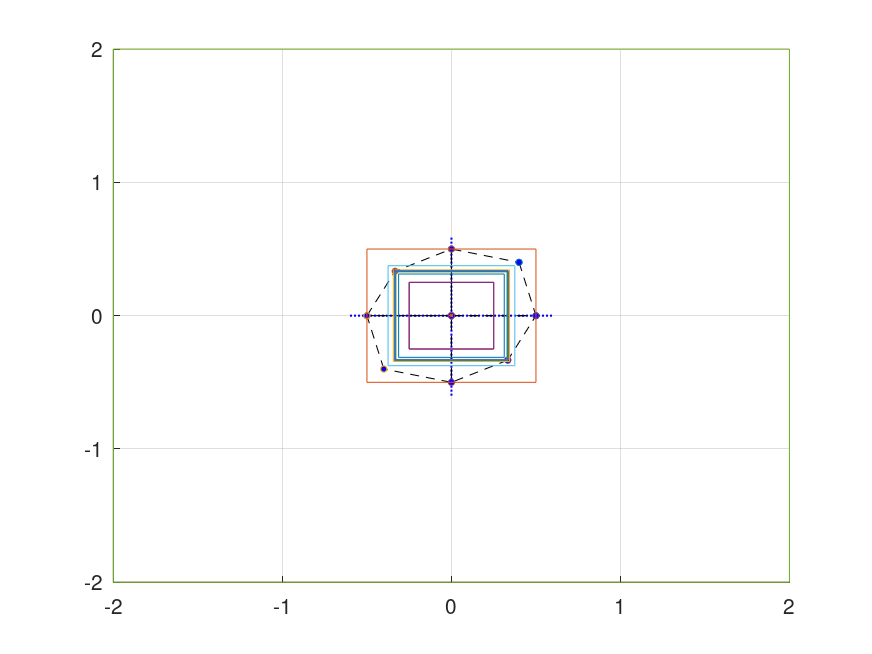
\includegraphics[width=0.8\textwidth]{Graphics/Decomp_boxes.png}
\caption{Работа схемы, основанной на теореме Зюзина} 
\end{figure}
\begin{figure}[H]\label{ZuzRad}
\centering
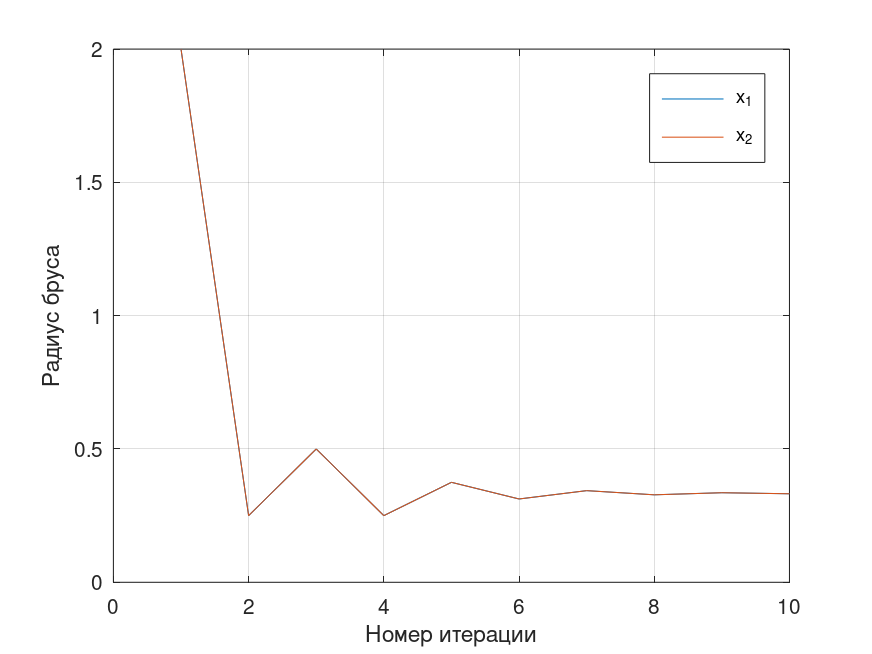
\includegraphics[width=0.8\textwidth]{Graphics/Decomp_radius.png}
\caption{Радиусы брусов при работе схемы, основанной на теореме Зюзина} 
\end{figure}
\subsection{Субдифференциальный метод Ньютона}
\begin{figure}[H]
\centering
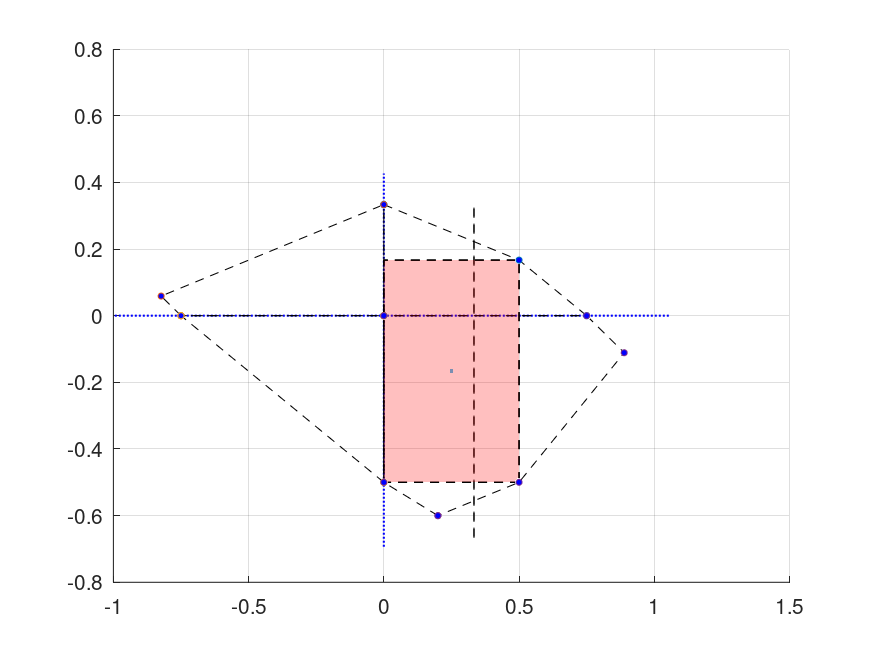
\includegraphics[width=0.8\textwidth]{Graphics/Newton1_boxes.png}
\caption{Работа cубдифференциального метода Ньютона для \eqref{System1}} 
\end{figure}
Алгоритм закончил свою работу на брусе $\begin{pmatrix}
    [   0,   0.5] \\
    [   -0.5,   0.16] \end{pmatrix}$, который обозначен на рисунке красным цветом.
\begin{figure}[H] \label{Cycle}
\centering
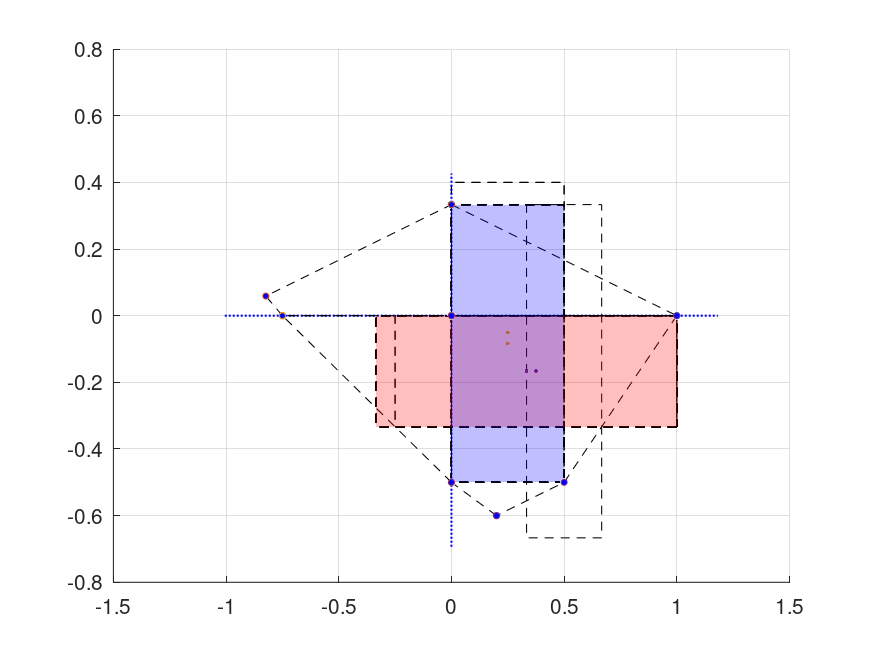
\includegraphics[width=0.8\textwidth]{Graphics/Newton2_boxes.png}
\caption{Работа cубдифференциального метода Ньютона для \eqref{System2}} 
\end{figure}
Алгоритм зациклился между двумя брусьями $-\,\begin{pmatrix}
    [   -0.3333,   1] \\
    [   -0.3333,   0] \end{pmatrix}$ и $\begin{pmatrix}
    [   0,   0.5] \\
    [   -0.5,   0.3333] \end{pmatrix}$, которые обозначены на рисунке красным и  синим цветом соответственно.